\documentclass[a4paper,12pt,titlepage]{article}
%\usepackage[T1]{fontenc}

\usepackage{titlesec}
\usepackage{titling}
\usepackage[portuguese]{babel}
\usepackage[utf8x]{inputenc}
\usepackage{indentfirst}
\usepackage{graphicx}
%\usepackage{times}
\usepackage{ucs}
\usepackage{float}    
\usepackage{fancyvrb}   
\usepackage{verbatim}
\usepackage{listings}
\usepackage{hyperref}
\usepackage{epigraph}
\usepackage{listings}
\usepackage{tabularx}
\usepackage{lipsum}

\hypersetup{
    colorlinks=true,       
    linkcolor=black,          
    citecolor=black,   
    filecolor=black,  
    urlcolor=black  
}

\hyphenation {di-re-cio-na-men-to} 

%\renewcommand*{\familydefault}{\ttdefault}
\lstset{columns=fullflexible,basicstyle=\ttfamily}

\title{\large
Universidade Federal de Minas Gerais \\ \
Instituto de Ciências Exatas \\ \ 
Departamento de Ciência da Computação \\ \
\\[1cm]
Projeto de Final de Curso\\ \
Projeto e Análise de Algoritmos\\ \
\\[1cm]
\textbf{\Large Modelagem, Baseline \\ e Plano de Experimentos }
\\[1cm]
}

\author{\large Alberto Hideki Ueda \\[0.5cm] 
	Orientador: Berthier Ribeiro Neto 
\\[3cm] }

\date{\textsc{Belo Horizonte\\ \
2 de novembro de 2014}}

\begin{document}
\maketitle

\pagebreak

\section{Contexto do Problema}

Coletores de páginas da \textit{Web} constituem o primeiro passo para a implementação de máquinas de busca modernas. De forma geral, um coletor - em inglês, \textit{crawler} - é um sistema que faz requisições a servidores da \textit{Web} de forma planejada e automática, coleta parte ou todo o conteúdo das páginas devolvidas pelas requisições e utiliza este novo conteúdo para realizar novas requisições \cite{b}. Estima-se que hoje mais de 10\% das visitas a \textit{Websites} sejam feitas por coletores \cite{nielsen}.

Hoje, mesmo as principais máquinas de busca cobrem apenas uma parte da \textit{Web} atual. Em 2005, foi demonstrado que o nível de cobertura das principais máquinas de buscas existentes está entre 58\% e 76\% da \textit{Web} \cite{gulli}. Além disso, o custo da utilização da rede também deve ser considerado. Em 2004, tal custo foi estimado em US\$ 1,5 milhão para coletores de larga escala \cite{craswell}. 

A ideia deste trabalho é modificar um algoritmo existente de um coletor genérico (\textit{General Crawler}) e transformá-lo em um coletor temático (\textit{Focused Crawler}) - que concentra-se em um único tópico de interesse - visando aumentar tanto a qualidade quanto a cobertura das páginas coletadas em relação ao algoritmo original.

Mais especificamente, este trabalho consistirá em alterações no escalonamento de longo prazo de um \textit{General Crawler}, direcionando as requisições de \textit{downloads} para páginas relevantes a um tópico pré-estabelecido, por meio de consultas de referência (\textit{driving queries}) ou documentos de exemplo (como um conjunto de páginas \textit{Web}).


\section{Modelagem}
Considerando as páginas da \textit{Web} como vértices e os diversos \textit{links} encontrados como arestas, pode-se aplicar diferentes algoritmos para a seleção \textit{on-line} (em tempo de execução) dos \textit{links} que o nosso \textit{focused crawler} irá visitar em um nova coleta. Possíveis estratégias de escolha (\textit{selection policy}) para o coletor baseiam-se, por exemplo, em: buscas em largura \cite{najork}, indicador \textit{PageRank} \cite{cho} ou até mesmo no uso de algoritmos genéticos \cite{johnson}. 

Levando-se em conta que não é possível coletar todas as páginas da \textit{Web}, devido à enorme quantidade de páginas e sua característica mutável, é importante encontrar as páginas mais relevantes o quanto antes. Quanto mais rápido uma página muito relevante for encontrada (de acordo com o indicador considerado), melhor a qualidade dos resultados obtidos em um dado instante de tempo da execução do coletor.

Logo, considerar a estrutura da \textit{Web} é interessante para a implementação de um \textit{crawler} de alto desempenho. Tal estrutura pode ser analisada sob duas perspectivas: \textit{microscópica} e \textit{macroscópica}.

Sob uma perspectiva microscópica, percebe-se que a estrutura dos \textit{links} não se assemelha a um arranjo aleatório. Ao invés disso, é comum identificar \textit{hubs} e redes \textit{scale-free} {\cite{barabasi}}, como ilustrado na figura abaixo.
\\ \ 

\begin{figure}[H]
     \centering
     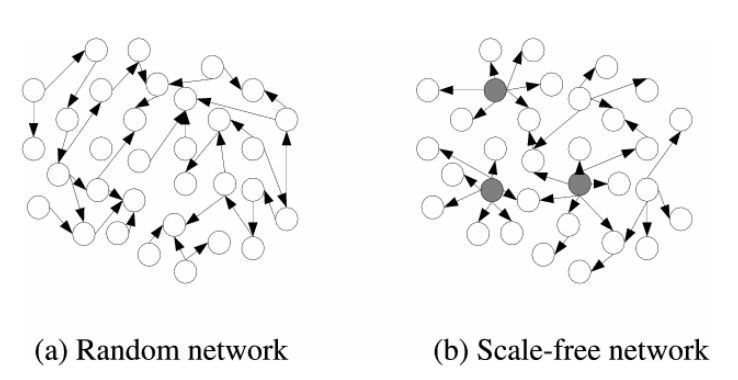
\includegraphics[scale=0.5]{figures/network-types.png}
     \caption{Exemplos de estruturas microscópicas da \textit{Web}. Uma rede gerada aleatoriamente (à esquerda) e uma rede \textit{scale-free} \cite{barabasi}.}
     \label{bsp}
\end{figure}

Já sob a perspectiva macroscópica, podemos identificar uma estrutura \textit{bow-tie} {\cite{broder}}, conforme visto em um dos trabalhos práticos da disciplina. A figura a seguir apresenta uma possível visualização desta estrutura.
 
\begin{figure}[H]
     \centering
     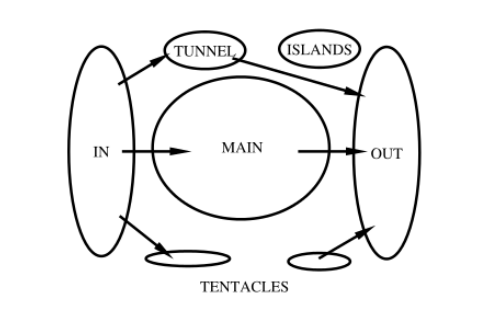
\includegraphics[scale=0.7]{figures/macroscopic-structure-web.png}
     \caption{Estrutura macroscópia da \textit{Web} \cite{broder}.}
     \label{bsp}
\end{figure}

Devido a estas perspectivas, muitos \textit{crawlers} são implementados de modo a beneficiar-se destas informações. Este é o caso do WIRE \cite{carlos}, o \textit{general web crawler} que é nosso \textit{baseline} para este trabalho. 

De forma geral, os coletores podem ser divididos em diversas categorias, conforme mostra a figura a seguir. Em cada categoria é possível identificar quais critérios são os mais importantes em uma coleta. É importante notar que um coletor genérico deve equilibrar todos os critérios apresentados, enquanto para um coletor temático a relevância das páginas e o quanto estão atualizadas são os critérios mais importantes, podendo haver detrimento do critério de representação (o quanto a página coletada reproduz o conteúdo original). 
\\ \ 

\begin{figure}[H]
     \centering
     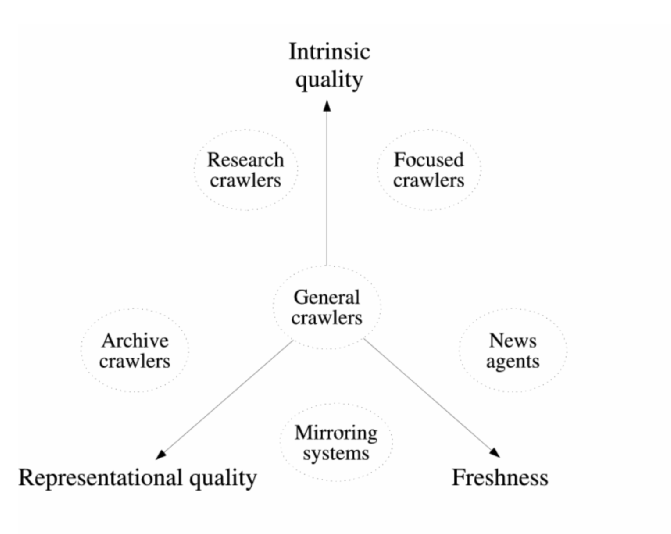
\includegraphics[scale=0.4]{figures/crawlers-types.png}
     \caption{Tipos de coletores \cite{carlos}.}
     \label{bsp}
\end{figure}



\section{Baseline}

O \textit{baseline} para este trabalho é o \textit{WIRE}, um \textit{general web crawler} desenvolvido por Carlos Castillo em seu doutorado na Universidade do Chile \cite{carlos}. Este coletor foi construído visando-se alto desempenho e boa escalabilidade, respeitando as políticas de restricões a visitas de robôs a servidores \textit{Web}.

O \textit{WIRE} foi desenvolvido para realizar integrações com máquinas de busca, como é comum no caso de coletores \textit{web}. A figura a seguir mostra o ciclo de funcionamento de um sistema completo, desde a coleta até a busca em si.

\begin{figure}[H]
     \centering
     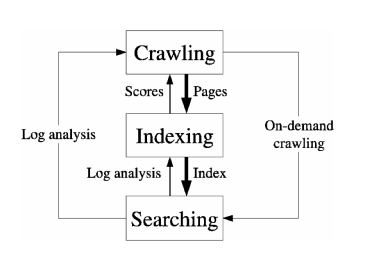
\includegraphics[scale=0.3]{figures/search-engine-cycle.png}
     \caption{Ciclo de uma máquina de busca \cite{carlos}.}
     \label{bsp}
\end{figure}

\ \\

O objetivo principal do \textit{WIRE} é realizar a caracterização da \textit{Web}, a partir dos dados coletados pelo \textit{crawler}. A figura abaixo encontra-se na tese de doutorado em que o \textit{WIRE} foi proposto. Ela mostra trabalhos futuros que podem utilizar este coletor, representados em cinza claro. Nota-se que o objetivo de nosso trabalho (construir um \textit{focused crawler}) está entre os itens citados.

\begin{figure}[H]
     \centering
     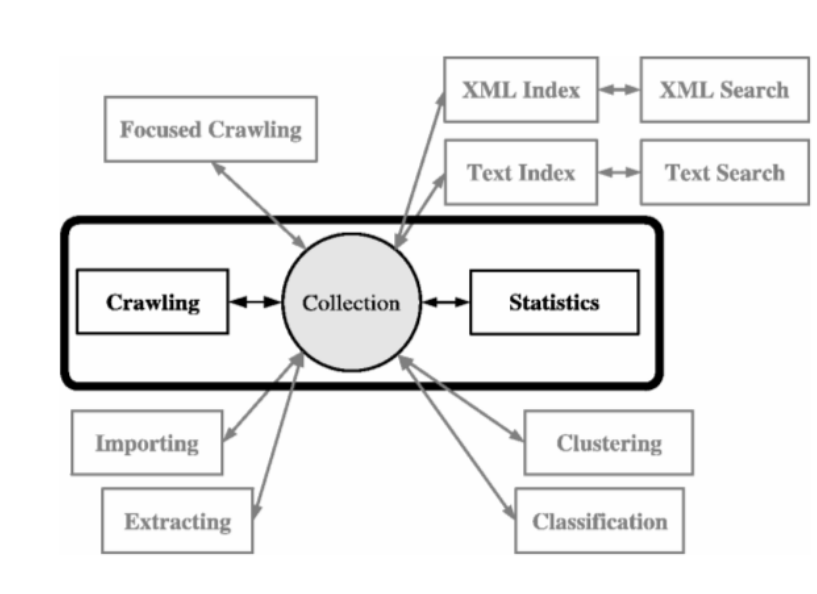
\includegraphics[scale=0.6]{figures/wire-architecture.png}
     \caption{Áreas de atuação do \textit{WIRE} (em preto) e trabalhos futuros (em cinza) \cite{carlos}.}
     \label{bsp}
\end{figure}

\subsection{Algoritmo}

O algoritmo deste \textit{baseline} é representado em alto nível pela figura a seguir.

\begin{figure}[H]
     \centering
     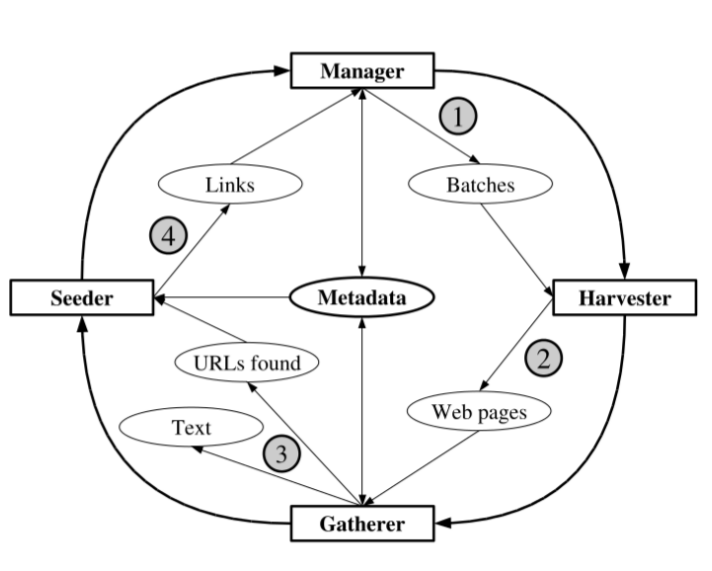
\includegraphics[scale=0.45]{figures/wire-crawling-architecture-2.png}
     \caption{Representação do funcionamento do coletor \textit{WIRE} \cite{carlos}.}
     \label{bsp}
\end{figure}

Cada componente é descrito a seguir: 

\begin{itemize}
\item \textit{Manager}: realiza os cálculos da relevância de cada página coletada e as atualizações no escalonamento de longo-prazo;
\item \textit{Harvester}: responsável pelo escalonamento de curto prazo e pelas coletas de páginas;
\item \textit{Gatherer}: faz o \textit{parse} e a extração de \textit{links};
\item \textit{Seeder}: responsável pela \textit{resolução} de \textit{URLs} e atualizações no grafo de \textit{links};
\end{itemize} 

O algoritmo utiliza listas de adjacências para representar a estrutura de \textit{links} encontrada entre as páginas, podendo ser descrito da seguinte forma:

\begin{enumerate}
\item (\textit{Seeder}) A partir de um arquivo inicial de \textit{URLs}, gera-se a lista das próximas páginas que devem ser coletadas;
\item (\textit{Manager}) Se uma página da lista gerada já foi visitada recentemente, a mesma é ignorada;
\item O valor intrínseco de cada página da lista é calculado, por meio de um indicador. Por exemplo, o \textit{PageRank} \cite{pagerank};
\item Calcula-se o quanto as páginas estão atualizadas;
\item Com o valor intrínseco e o nível de atualização das páginas, calcula-se a qualidade geral de cada página;
\item Extrai-se então da lista as $k$ páginas de maior qualidade, $k$ determinado em um arquivo de configuração;
\item (\textit{Harvester}) Determina-se como as $k$ páginas serão coletadas (observando regras de "bom comportamento" para coletores);
\item Coleta-se todas as páginas de acordo com as regras determinadas no item anterior;
\item (\textit{Gatherer}) As informações coletadas são tratadas, armazenando-se o que é relevante e descartando o restante do material coletado;
\item São enviadas para o (\textit{Seeder}) as novas \textit{URLs} encontradas nas páginas coletadas e reinicia-se o processo, agora sem a necessidade de arquivos de inicialização;
\end{enumerate}

A condição de parada depende do objetivo do usuário, que pode priorizar cobertura (continuar até que não haja páginas no domínio de interesse, demandando potencialmente um tempo inviável) ou por critério de tempo (encerra-se quando atingir um nível determinado de cobertura). O estudo do \textit{WIRE} mostrou que a partir de uma coleta com 50\% de uma grande coleção de páginas, já é possível atingir 80\% do valor total do \textit{PageRank} dessa coleção \cite{carlos}.


\section{Plano de Experimentos}

O objetivo deste trabalho é transformar o \textit{general web crawler} de referência em um \textit{focused crawler}, melhorando os resultados obtidos pelo coletor original, dado um tema específico. Para isso, modificaremos a estratégia que um coletor genérico utiliza para determinar quais são os próximos \textit{links} que devem ser processados. No caso do \textit{WIRE}, devemos alterar seu escalonamento de longo-prazo (componente \textit{manager}, conforme seção anterior), substituindo parte do código por um novo algoritmo de escolha das próximas páginas que deverão ser coletadas.

Em seguida, executaremos testes de coleta para os dois algoritmos - original e modificado - e faremos a comparação dos resultados obtidos. Dado um tópico-alvo para a coleta, espera-se que o algoritmo adaptado seja melhor em termos de espaço e memória que o original. Mais especificamente, o \textit{focused crawler} deverá encontrar as páginas mais relevantes antes do \textit{crawler} genérico. Parte das mesmas métricas utilizadas para avaliar o \textit{WIRE} serão aplicadas para o nosso coletor e os resultados serão apresentados.

Na tese de doutorado de Carlos Castillo, diferentes estratégias foram testadas para se medir o desempenho do \textit{WIRE}. Nenhuma leva em conta o caráter temático do coletor, já que o objetivo de seu trabalho era a implementação de um \textit{crawler} de uso geral.
Porém, pode-se ter uma ideia do que esperamos com nosso trabalho visualizando o gráfico a seguir, obtido da tese em que o \textit{WIRE} foi apresentado. Para cada estratégia (linha), quanto antes a mesma atingir o \textit{PageRank} \cite{pagerank} máximo (igual a 1), melhor é a estratégia, como dito na seção de modelagem. Dado um tema específico, nosso \textit{focused crawler} poderá ser representado por uma nova linha no gráfico. É desejado que a mesma esteja acima (encontre as páginas mais relevantes antes) das estratégias do \textit{crawler} original.



\begin{figure}[H]
     \centering
     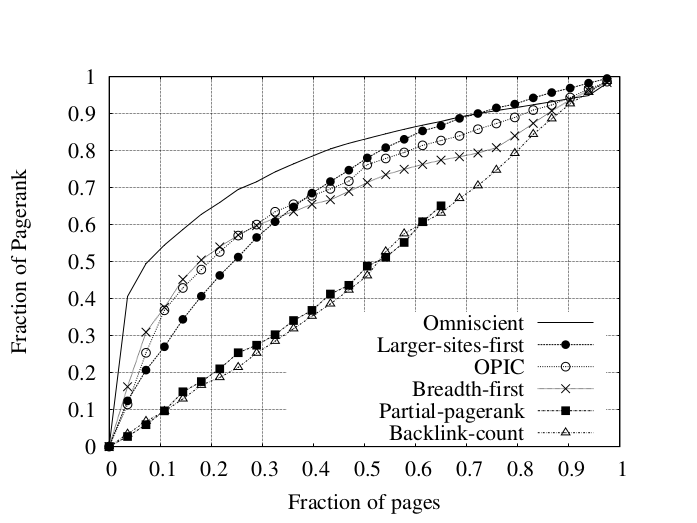
\includegraphics[scale=0.6]{figures/performance.png}
     \caption{Gráfico com os desempenhos de diferentes estratégias para escalonamento de longo prazo  \cite{carlos}.}
     \label{bsp}
\end{figure}



% Referências
\bibliographystyle{plain}%amsalpha
\bibliography{bibliografia}
\newpage

\end{document}


